\part{Алгебра}   
\chapter{Элементарная}
\section{Рациональные выражения}
\subsection{Формулы сокращённого умножения}
\begin{itemize}
	\item $(a \pm b)^n$ вычисляется через треугольник паскаля\\
	\begin{center}
		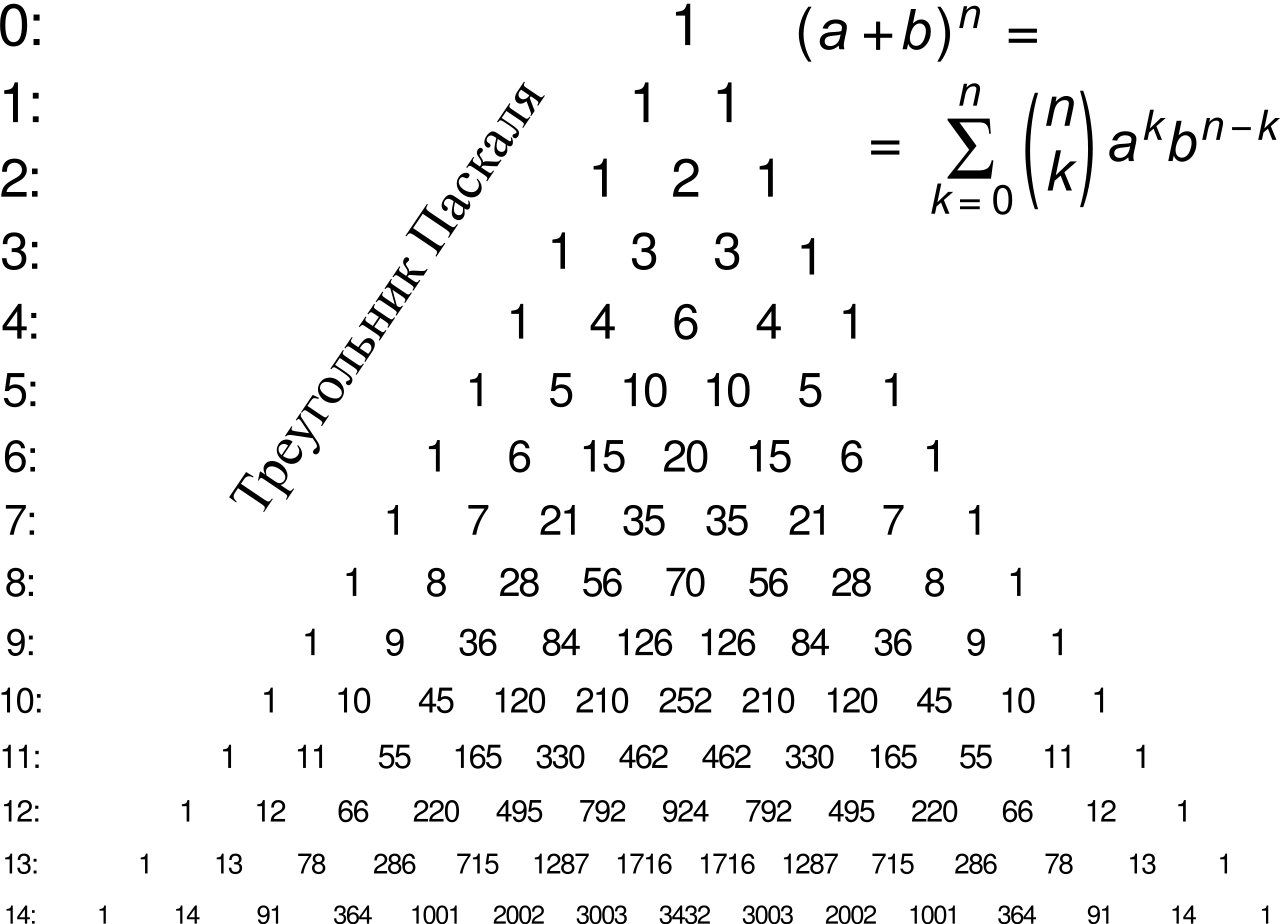
\includegraphics[scale=0.2]{./mh/algebra/elementary/rational_expressions/Pascal_triangle.png}
	\end{center}
	Например:\\
	\begin{itemize}
		\item 
	\end{itemize}
\end{itemize}          
\chapter{Общая алгебра}
\index{алгебраическая структура}\textbf{Алгебраическая структура} - это множество элементов с определёнными на них операциями. Определение алгебраической структуры можно записать как набор значений в скобках.
Например $(M, +, *)$ - алгебраическая структура с определёнными операциями сложения и умножения.

% 1 лекция 
% операторы унарные бинарные тернарные ..
% операции сложения и умножения, противоположные и обратные элементы (нейтральные), аддитивная и мультипликативная запись
% ассоциативность и коммутативность
% инфиксная запись, постфиксная префиксная интерфиксная запись
% 2 лекция
% моноиды, регулярные справа и слева элем, обратимые элементы

Операнд - аргумент операции.

Операция $\circ$ в множестве $M$ - это какое то отображение $M \circ M  \rightarrow M$. В алгебре обычно принято записывать операции в виде инфиксной записи (оператор пишется между операндами, например $a + b$).

Если $\forall a,b,c \in M : (a \circ b) \circ c = a \circ (b \circ c)$, то говорят, что $\circ$ -  \index{ассоциативная операция}\textbf{ассоциативная операция}.

Если $\forall a,b \in M : a \circ b = b \circ a$, то говорят, что $\circ$ - \index{коммутативная операция}\textbf{коммутативная операция}.

Пусть $M$ - множество с операцией $\circ$, а $N$ - множество с операцией $*$. Алгебраические структуры $(M, \circ)$ и $($N$, *)$ называют \textbf{изоморфными}, если существует такое биективное отображение
$$
f: M \rightarrow N
$$
что
$$
f(a \circ b) = f(a) * f(b)
$$
где $a, b \in M$. В этом случае говорят $(M, \circ) \simeq ($N$, *)$. Само отображение $f$ называют \index{изоморфизм!алгебраических структур} \textbf{изоморфизмом}.

\index{нейтральный элемент}\textbf{Нейтральный элемент} множества $M$  с операцией $\circ$ - это такой элемент $e \in M$, что $\forall x \in M : x \circ e = e \circ x = x$.


\index{аддитивная запись}\textbf{Аддитивная запись} - запись через оператор сложения$\mathbf{+}$. $0$ \textbf{(Ноль)} - это нейтральный элемент при аддитивной записи, то есть $x + 0 = 0 + x = 0$. 

Элемент $x'$ для элемента $x$ называется противоположным справа, если $x + x' = 0$.

Элемент $x'$ для элемента $x$ называется противоположным слева, если $x' + x = 0$.

Элемент $x'$ для элемента $x$ называется \index{противоположный элемент}\textbf{противоположным}, если $x + x' = x' + x = 0$. Так же элемент, противоположный $x$ обозначается как $-x$.


\index{мультипликативная запись}\textbf{Мультипликативная запись} - запись через оператор умножения $\mathbf{*}$. $1$ \textbf{(Единица)} - это нейтральный элемент при аддитивной записи, то есть $x * 1 = 1 * x = 1$. 

Элемент $x'$ для элемента $x$ называется обратным справа, если $x * x' = 1$.

Элемент $x'$ для элемента $x$ называется обратным слева, если $x' * x = 0$.

Элемент $x'$ для элемента $x$ называется \index{обратный элемент}\textbf{обратным}, если $x * x' = x' * x = 0$. Так же элемент, обратным $x$ обозначается как $x^{-1}$.

\index{обратимый элемент}\textbf{Обратимый элемент} - это элемент, для которого существует обратный.

\section{Группы}
\index{полугруппа}\textbf{Полугруппа} - это множество с заданной на нём ассоциативной бинарной операцией $(S, *)$.

\index{моноид}\textbf{Моноид} - это полугруппа с единицей.

\textbf{Группа} - это такая алгебраическая структура $(S, *, -1, 1)$, для которой выполняется три свойства:
\begin{enumerate}
	\item $*$ задаёт операцию на множестве $S$.
	\item Существование обратного элемента $\forall x \in S \quad \exists x^{-1}$
	\item Существование единицы.
\end{enumerate} 

\index{аддитивная абелева группа}\textbf{Аддитивная абелева группа} - это множество с заданной на нём операцией сложения $(S, +)$ и обладающее свойствами коммутативности и ассоциативности, существования нуля (единственного) и существования для каждого элемента (единственного) противоположного ему.

\index{мультипликативная абелева группа}\textbf{Мультипликативная абелева группа} - это множество с заданной на нём операцией умножения $(S, *)$ и обладающее свойствами коммутативности и ассоциативности, существования единицы (единственной) и существования для каждого элемента (единственного) обратного ему.




\section{Теория колец}

\index{кольцо}\textbf{Кольцо} - это алгебраическая структура с операциями сложения и умножения $(S, +, *)$, обладающая следующими свойствами:
\begin{enumerate}
	\item Относительно сложения это аддитивная абелева группа.
	
	\item Выполняется дистрибутивность умножения относительно сложения, то есть $\forall a, b, c \in S : a*(b+c) = a*b + a*c$. 
\end{enumerate}

Кольцо называется ассоциативным, если умножение в нём ассоциативно.

Кольцо называется коммутативным, если умножение в нём коммутативно.

\section{Поля}
\index{поле}\textbf{Полем} называется коммутативное ассоциативное кольцо с единицей, в котором всякий ненулевой элемент обратим.

Примеры полей: $\mathbb{R}$, $\mathbb{Q}$.	
  
\chapter{Линейная алгебра}
\section{Линейные комбинации}
Выражение, построенное на~множестве элементов путём сложения этих элементов, умноженных на~некоторые коэффициенты, называется \textbf{линейной комбинацией}.
Если все коэффициенты линейной комбинации равны нулю, то она называется \textbf{тривиальной}, иначе~--- \textbf{нетривиальной}.
\section{Матрицы}
\textbf{Матрицей} называется прямоугольная таблица из~чисел, содержащая $m$~строк и~$n$~столбцов, и~обозначается
\begin{equation*}
A =
\begin{pmatrix}
a_{11} & a_{12} & \cdots & a_{1n} \\
a_{21} & a_{22} & \cdots & a_{2n} \\
\vdots & \vdots & \ddots & \vdots \\
a_{m1} & a_{m2} & \cdots & a_{mn}
\end{pmatrix} =
\begin{Vmatrix}
a_{11} & a_{12} & \cdots & a_{1n} \\
a_{21} & a_{22} & \cdots & a_{2n} \\
\vdots & \vdots & \ddots & \vdots \\
a_{m1} & a_{m2} & \cdots & a_{mn}
\end{Vmatrix}
\end{equation*}

Числа $m$ и~$n$ называются \textbf{порядками} матрицы.

Если $m = n$, то матрица называется \textbf{квадратной}, а число~$m = n$~--- её \textbf{порядком}.
\textbf{Главной} называется диагональ квадратной матрицы, состоящая из~элементов $a_{11}, a_{22}, \ldots, a_{nn}$, а \textbf{побочной}~--- состоящая из~элементов $a_{n1}, a_{n-1\, 2}, \ldots, a_{1n}$.

$i$\nobreakdash-я строка матрицы обозначается~$A_i$, $j$\nobreakdash-й столбец~---~$A^j$.

Две матрицы называются \textbf{равными}, если их порядки и~соответствующие элементы совпадают, иначе~--- \textbf{неравными}.
% \section{Векторные пространства}
$n$\nobreakdash-мерным векторным пространством над~полем вещественных чисел называется множество
\begin{equation*}
V_n = \mathbb R^n = \{ (x_1; \ldots; x_n) \mid x_1, \ldots, x_n \in \mathbb R \}
\end{equation*}
элементы которого называются \textbf{векторами}. Над~ними определены операции сложения и~умножения на число, удовлетворяющие аксиомам:
\begin{enumerate}
	\item Коммутативность сложения:
	\begin{equation*}
	\forall \overline a, \overline b \in V_n \ 
	\overline a + \overline b = \overline b + \overline a
	\end{equation*}
	
	\item Ассоциативность сложения:
	\begin{equation*}
	\forall \overline a, \overline b, \overline c \in V_n \ 
	\overline a + (\overline b + \overline c) = (\overline a + \overline b) + \overline c
	\end{equation*}
	
	\item Существование \textbf{нулевого} вектора, или~\textbf{нуля}, обозначаемого $\overline 0$:
	\begin{equation*}
	\exists \overline 0 \in V_n \colon \forall \overline a \in V \ 
	\overline a + \overline 0 = \overline 0 + \overline a = \overline a
	\end{equation*}
	
	\item Существование \textbf{противоположного} вектора:
	\begin{equation*}
	\forall \overline a \in V_n \ 
	\exists (-\overline a) \in V_n \colon
	\overline a + (-\overline a) = \overline 0
	\end{equation*}
	
	\item Ассоциативность умножения на~число:
	\begin{equation*}
	\forall \alpha, \beta \in \mathbb R, \ 
	\forall \overline a \in V_n \ 
	\alpha (\beta \overline a) = (\alpha \beta) \overline a
	\end{equation*}
	
	\item Дистрибутивность умножения на~число относительно сложения векторов:
	\begin{equation*}
	\forall \alpha \in \mathbb R, \ 
	\forall \overline a, \overline b \in V_n \ 
	\alpha (\overline a + \overline b) = \alpha \overline a + \alpha \overline b
	\end{equation*}
	
	\item Дистрибутивность умножения на~число относительно сложения чисел:
	\begin{equation*}
	\forall \alpha, \beta \in \mathbb R, \ 
	\forall \overline a \in V_n \ 
	(\alpha + \beta) \overline a = \alpha \overline a + \beta \overline a
	\end{equation*}
	
	\item Существование \textbf{единицы}:
	\begin{equation*}
	\forall \overline a \in V_n \ 
	1 \cdot \overline a = \overline a
	\end{equation*}
\end{enumerate}
% beta
\section{Системы линейных алгебраических уравнений}
\index{СЛАУ|see{cистема линейных алгебраических уравнений}}\index{cистема линейных алгебраических уравнений}\textbf{Система линейных алгебраических уравнений (СЛАУ)} имеет вид
\begin{equation*}
\begin{cases}
a_{11}x_1 + a_{12}x_2 + \dots + a_{1n}x_n = b_1 \\
a_{21}x_1 + a_{22}x_2 + \dots + a_{2n}x_n = b_2 \\
\vdots \\
a_{m1}x_1 + a_{m2}x_2 + \dots + a_{mn}x_n = b_m
\end{cases}
\end{equation*}
где $x_1, \ldots, x_n$~--- переменные.

$a_{11}, a_{12}, \ldots, a_{mn}$ называются \textbf{коэффициентами при~переменных}, $b_1, b_2, \dots, b_m$~--- \textbf{свободными членами}.

\textbf{Решение системы линейных уравнений} это такой вектор $(x_1, \ldots, x_n)$, что при подстановки его его значений заместо переменных мы получаем верную систему.

Система линейных уравнений называется \index{СЛАУ!однородная}\textbf{однородной}, если все её свободные члены равны 0, иначе~--- \index{СЛАУ!неоднородная}\textbf{неоднородной}.

Система линейных уравнений называется \index{СЛАУ!совместная}\textbf{совместной}, если она имеет хотя~бы одно решение, иначе~--- \index{СЛАУ!несовместная}\textbf{несовместной}.

Система линейных уравнений называется \index{СЛАУ!определённая}\textbf{определённой}, если она имеет единственное решение.
Если система имеет более одного решения, то она называется \index{СЛАУ!неопределённая}\textbf{неопределённой}.

Две системы линейных уравнений называются \index{СЛАУ!эквивалентная}\textbf{эквивалентными}, если их решения совпадают или~обе не~имеют решений.

Строки СЛАУ можно рассматривать как элементы некоторого векторного пространства над полем $K$, а саму СЛАУ как множество этих элементов. Строку СЛАУ можно рассматривать как такой вектор $(a_1, \cdot a_n, b)$, который задаёт выражение от $n$-переменным $a_1 x_1 + \cdot + a_n x_n = b$.

\begin{theorem}
	Пусть $V$ - множество векторов, которое задаёт СЛАУ, и $V'$ - СЛАУ, полученная из $V$ заменой какого-то элемента на линейную комбинацию других. Тогда $V$ и $V'$ - эквивалентны.
\end{theorem}
\begin{proof}
	Пусть $s_k = (a_{1k}, \cdot a_{nk}, b_k)$ - любая строка $V$, $s'_k$ - строка, полученная линейной комбинацией других строк. Теперь докажем, что множество решений для строки $s_k$ совпадает с множеством решений $s'_k$. Возьмём любое решение $(x_1, \ldots, x_n)$ для $s_k$ и поставим в $s'_k$ как в уравнение. Пользуюсь тем, что $K$ - это поле, элементами векторного пространства над которым являются $s'_k$ и $s_k$, получим верное верное равенство. Аналогично доказывается то, что все решения $s'_k$ яв-ся решениями $s_k$.
\end{proof}

\subsection{Матричная форма системы линейных уравнений}
Систему линейных уравнений можно представить в матричной форме:
\begin{equation*}
\begin{Vmatrix}
a_{11}x_1 + a_{12}x_2 + \dots + a_{1n}x_n \\
a_{21}x_1 + a_{22}x_2 + \dots + a_{2n}x_n \\
\vdots \\
a_{m1}x_1 + a_{m2}x_2 + \dots + a_{mn}x_n
\end{Vmatrix} =
\begin{Vmatrix}
b_1 \\
b_2 \\
\vdots \\
b_m
\end{Vmatrix}
\Leftrightarrow
\end{equation*}
\begin{equation*}
\Leftrightarrow
\begin{Vmatrix}
a_{11} & a_{12} & \cdots & a_{1n} \\
a_{21} & a_{22} & \cdots & a_{2n} \\
\vdots & \vdots & \ddots & \vdots \\
a_{m1} & a_{m2} & \cdots & a_{mn}
\end{Vmatrix} \cdot
\begin{Vmatrix}
x_1 \\
x_2 \\
\vdots \\
x_n
\end{Vmatrix} =
\begin{Vmatrix}
b_1 \\
b_2 \\
\vdots \\
b_m
\end{Vmatrix}
\Leftrightarrow
\end{equation*}
\begin{equation*}
\Leftrightarrow
A \cdot X = B
\end{equation*}

$A$ называется \textbf{основной матрицей системы}, $X$~--- \textbf{столбцом переменных}, $B$~--- \textbf{столбцом свободных членов}.
Если к основной матрице справа приписать столбец свободных членов, то получится \textbf{расширенная матрица системы}:
\begin{equation*}
\begin{Vmatrix}
a_{11} & a_{12} & \cdots & a_{1n} & \vline & b_1 \\
a_{21} & a_{22} & \cdots & a_{2n} & \vline & b_2 \\
\vdots & \vdots & \ddots & \vdots & \vline & \vdots \\
a_{m1} & a_{m2} & \cdots & a_{mn} & \vline & b_m
\end{Vmatrix}
\end{equation*}
% beta
\subsection{Линейная независимость}
Уравнение системы линейных уравнений называется \textbf{линейно зависимым}, если соответствующая ему строка расширенной матрицы является нетривиальной линейной комбинацией других строк, иначе~--- \textbf{линейно независимым}.

Система линейных уравнений называется \textbf{линейно зависимой}, если существует нетривиальная линейная комбинация строк расширенной матрицы, в~результате которой получается нулевая строка, иначе~--- \textbf{линейно независимой}.

\begin{statement}
Система линейных уравнений линейно зависима $\Leftrightarrow$ одно из~её уравнений линейно зависимо.
\end{statement}
\begin{proof}
\begin{enumerate}
	\item $\Rightarrow$. Пусть система из строк $A_1, \ldots, A_n$ линейно зависима:
	\begin{equation*}
	\sum_{i=1}^n \alpha_i A_i = O, \ \sum_{i=1}^n \alpha_i^2 \neq 0
	\end{equation*}
	где $O$~--- нулевая строка. Без ограничения общности можно считать, что $\alpha_1 \neq 0$, тогда
	\begin{equation*}
	A_1 = -\sum_{i=2}^n \frac{\alpha_i}{\alpha_1} A_i
	\end{equation*}
	
	Значит, $A_1$~--- линейно зависимая строка.
	
	\item $\Leftarrow$. Пусть одна из строк линейно зависима:
	\begin{equation*}
	A_1 = \sum_{i=2}^n \alpha_i A_i \Leftrightarrow
	1 \cdot A_1 - \alpha_2 A_2 - \ldots - \alpha_n A_n = O
	\end{equation*}
	
	Значит, система линейно зависима.
\end{enumerate}
\end{proof}
% beta
\subsection{Решение систем линейных уравнений}
\begin{lemma}
Пусть система из~строк $A_1, \ldots, A_n$ линейно независима и~$A_{n+1}$ не~является линейной комбинацией $A_1, \ldots, A_n$. Тогда система из~строк $A_1, \ldots, A_n, A_{n+1}$ линейно независима.
\end{lemma}
\begin{proofcontra}
Пусть система из~строк $A_1, \ldots, A_n, A_{n+1}$ линейно зависима:
\begin{equation*}
\sum_{i=1}^{n+1} \alpha_i A_i = O, \ 
\sum_{i=1}^{n+1} \alpha_i^2 \neq 0
\end{equation*}
где $O$~--- нулевая строка.
Система из~строк $A_1, \ldots, A_n$ линейно независима по~условию, тогда
\begin{equation*}
\alpha_{n+1} \neq 0 \Rightarrow A_{n+1} = -\sum_{i=1}^n \frac{\alpha_i}{\alpha_{n+1}} A_i
\end{equation*}

Значит, $A_{n+1}$~--- линейная комбинация $A_1, \ldots, A_n$.
Противоречие с~условием.
\end{proofcontra}

\begin{theorem}[Кронекера~---~Капелли]
Система линейных уравнений совместна $\Leftrightarrow$ ранг основной матрицы совпадает с~рангом расширенной матрицы.
\end{theorem}
\begin{proof}
\begin{enumerate}
	\item $\Rightarrow$. 
	\item $\Leftarrow$.
\end{enumerate}
\end{proof}

\subsubsection{Метод Гаусса}
Пусть дана система линейных уравнений
\begin{equation}
\label{eq:Gaussian_elimination(1)}
\begin{cases}
a_{11}x_1 + a_{12}x_2 + \dots + a_{1n}x_n = b_1 \\
a_{21}x_1 + a_{22}x_2 + \dots + a_{2n}x_n = b_2 \\
\vdots \\
a_{m1}x_1 + a_{m2}x_2 + \dots + a_{mn}x_n = b_m
\end{cases}
\end{equation}

Её расширенную матрицу можно привести к~ступенчатому виду, т.\,е. (\ref{eq:Gaussian_elimination(1)}) эквивалентна
\begin{equation}
\label{eq:Gaussian_elimination(2)}
\begin{cases}
a_{1\, j_1} x_{j_1} + \ldots + a_{1\, j_n} x_{j_n} = b_1 \\
a_{2\, j_2} x_{j_2} + \ldots + a_{2\, j_n} x_{j_n} = b_2 \\
\vdots \\
a_{r\, j_r} x_{j_r} + \ldots + a_{r\, j_n} x_{j_n} = b_r \\
0 = b_{r+1} \\
\vdots \\
0 = b_m
\end{cases}
\end{equation}
где $a_{1\, j_1}, \ldots, a_{r\, j_r} \neq 0$.
Без~ограничения общности можно считать, что в~базисный минор основной матрицы системы (\ref{eq:Gaussian_elimination(2)}) входят только коэффициенты при~переменных $x_{j_1}, \ldots, x_{j_r}$, называемых \textbf{главными (зависимыми)}.
Остальные переменные называются \textbf{свободными (независимыми)}.

Если $\exists i > r \colon b_i \neq 0$, то система несовместна.
Пусть $\forall i > r \ b_i = 0$. Тогда получим систему
\begin{equation*}
\begin{cases}
\displaystyle x_{j_1} = \frac{b_1}{a_{1\, j_1}} - \frac{a_{1\, j_2}}{a_{1\, j_1}} x_{j_2} - \ldots - \frac{a_{1\, j_n}}{a_{1\, j_1}} x_{j_n} \\
\displaystyle x_{j_2} = \frac{b_2}{a_{2\, j_2}} - \frac{a_{2\, j_3}}{a_{2\, j_2}} x_{j_3} - \ldots - \frac{a_{2\, j_n}}{a_{2\, j_2}} x_{j_n} \\
\vdots \\
\displaystyle x_{j_r} = \frac{b_r}{a_{r\, j_r}} - \frac{a_{r\, j_{r+1}}}{a_{r\, j_r}} x_{j_{r+1}} - \ldots - \frac{a_{r\, j_n}}{a_{r\, j_r}} x_{j_n} \\
\end{cases}
\end{equation*}

Если свободным переменным полученной системы придавать все возможные значения и~решать новую систему относительно главных неизвестных от~нижнего уравнения к~верхнему, то получим все решения данной системы.

\subsubsection{Метод Крамера}
Позволяет решить только те системы, которые имеют единственное решение. Пусть дана система линейно независимых уравнений
\begin{equation*}
\begin{cases}
a_{11}x_1 + a_{12}x_2 + \dots + a_{1n}x_n = b_1 \\
a_{21}x_1 + a_{22}x_2 + \dots + a_{2n}x_n = b_2 \\
\vdots \\
a_{n1}x_1 + a_{n2}x_2 + \dots + a_{nn}x_n = b_n
\end{cases}
\end{equation*}

Определитель основной матрицы системы не~равен 0, т.\,к. строки линейно независимы. Запишем систему в~матричной форме:
\begin{equation*}
AX = B \Leftrightarrow
X = A^{-1}B \Leftrightarrow
\end{equation*}
\begin{equation*}
\Leftrightarrow
\begin{Vmatrix}
x_1 \\
x_2 \\
\vdots \\
x_n
\end{Vmatrix} =
\begin{Vmatrix}
\dfrac{A_{11}}{|A|} & \dfrac{A_{21}}{|A|} & \cdots & \dfrac{A_{n1}}{|A|} \\
\dfrac{A_{12}}{|A|} & \dfrac{A_{22}}{|A|} & \cdots & \dfrac{A_{n2}}{|A|} \\
\vdots & \vdots & \ddots & \vdots \\
\dfrac{A_{1n}}{|A|} & \dfrac{A_{2n}}{|A|} & \cdots & \dfrac{A_{nn}}{|A|}
\end{Vmatrix} \cdot
\begin{Vmatrix}
b_1 \\
b_2 \\
\vdots \\
b_n
\end{Vmatrix}
\end{equation*}
где $A_{ij}$~--- алгебраическое дополнение $a_{ij}$.

Т.\,о., получим решение системы:
\begin{equation*}
\label{eq:Cramer's_formula}
x_i = \frac{\sum_{j=1}^n A_{ji} b_j}{|A|} =
\frac{
\begin{vmatrix}
a_{11} & \cdots & a_{1\, i-1} & b_{1} & a_{1\, i+1} & \cdots & a_{1n} \\
a_{21} & \cdots & a_{2\, i-1} & b_{2} & a_{2\, i+1} & \cdots & a_{2n} \\
\vdots & \ddots & \vdots & \vdots & \vdots & \ddots & \vdots \\
a_{n1} & \cdots & a_{n\, i-1} & b_{n} & a_{n\, i+1} & \cdots & a_{nn} \\
\end{vmatrix}
}
{
|A|
}, \ i = 1, \ldots, n
\end{equation*}

Полученные формулы называется \textbf{формулами Крамера}.
% beta
\subsection{Фундаментальная система решений}
\begin{statement}
Однородная линейно независимая система уравнений
\begin{equation*}
\begin{cases}
\displaystyle \sum_{i=1}^n a_{1i} x_i = 0 \\
\displaystyle \sum_{i=1}^n a_{2i} x_i = 0 \\
\vdots \\
\displaystyle \sum_{i=1}^n a_{mi} x_i = 0
\end{cases}
\end{equation*}
задаёт векторное пространство размерности~$n - m$.
\end{statement}
\begin{proof}

\end{proof}

\textbf{Фундаментальной системой решений} однородной системы линейных уравнений называется базис множества всех её решений.

\subsubsection{Нахождение фундаментальной системы решений}
Пусть дана однородная линейно независимая система уравнений:
\begin{equation*}
\begin{cases}
\displaystyle \sum_{i=1}^n a_{1i} x_i = 0 \\
\displaystyle \sum_{i=1}^n a_{2i} x_i = 0 \\
\vdots \\
\displaystyle \sum_{i=1}^n a_{mi} x_i = 0 \\
\end{cases} \Leftrightarrow
\begin{cases}
\displaystyle \sum_{i=1}^m a_{1i} x_i = -\sum_{i=m+1}^n a_{1i} x_i \\
\displaystyle \sum_{i=1}^m a_{2i} x_i = -\sum_{i=m+1}^n a_{2i} x_i \\
\vdots \\
\displaystyle \sum_{i=1}^m a_{mi} x_i = -\sum_{i=m+1}^n a_{mi} x_i \\
\end{cases}
\end{equation*}

Пусть 
\begin{equation*}
(x_{11}; x_{21}; \ldots; x_{m1}; 1; 0; \ldots; 0)
\end{equation*}
\begin{equation*}
(x_{12}; x_{22}; \ldots; x_{m2}; 0; 1; \ldots; 0)
\end{equation*}
\begin{equation*}
\vdots
\end{equation*}
\begin{equation*}
(x_{1\, n-m}; x_{2\, n-m}; \ldots; x_{m\, n-m}; 0; 0; \ldots; 1)
\end{equation*}
являются решениями данной системы. 
Тогда они образуют фундаментальную систему решений.
\begin{proof}

\end{proof}

\begin{theorem}
Общее решение неоднородной системы линейных уравнений равно сумме её частного решения и~общего решения соответствующей однородной системы, т.\,е. с~теми~же самыми коэффициентами при~переменных.
\end{theorem}
\begin{proof}

\end{proof}
\section{Многочлены от одной переменной}
\textbf{Одночленом}, или \textbf{мономом}, называется произведение числового множителя и~нуля и~более переменных, взятых каждая в~неотрицательной степени.

\textbf{Степенью} одночлена называется сумма степеней входящих в~него переменных. Степень тождественного нуля равна $-\infty$.

\textbf{Многочленом}, или \textbf{полиномом}, от~одной переменной называется сумма вида
\begin{equation*}
a_0 + a_1 x + a_2 x^2 + \ldots + a_n x^n
\end{equation*}
где $x_1, \ldots, x_n$~--- переменные.

\textbf{Степенью} многочлена называется максимальная из~степеней его одночленов.

\begin{lemma}
Пусть $f$ и~$g$~--- многочлены, тогда $\deg fg = \deg f + \deg g$.
\end{lemma}
\section{Многочлены от нескольких переменных}
\begin{enumerate}
	\item В~многочлене $a_n x^n + a_{n-1} x^{n-1} + \ldots + a_0$ подставим $a_i = P_i(y)$~--- многочлен от~$y$.
	Получим многочлен от~$x$ и~$y$.
	
	\item Пусть имеем многочлен от~$n$~переменных.
	Подставим вместо его коэффициентов многочлен от~одной переменной, получим многочлен от~$n + 1$~переменных.
\end{enumerate}

Одночлены многочлена будем записывать в~лексикографическом порядке степеней переменных (члены с~б\'{о}льшими степенями идут раньше).

\begin{theorem}
Старший член произведения многочленов равен произведению старших членов множителей.
\end{theorem}
\begin{proof}
Перемножая члены с~наибольшими показателями старшей переменной, получим член с~наибольшим показателем при~этой переменной.
Проведя аналогичные рассуждения для~остальных переменной, придём к~выводу, что полученный член является старшим.
\end{proof}

Аналогично доказывается следующая теорема.
\begin{theorem}
Младший член произведения многочленов равен произведению младших членов множителей.
\end{theorem}
% beta
\section{Квадратные формы}
\textbf{Квадратичной формой} называется многочлен, все одночлены в~котором второй степени:
\begin{equation*}
f(x_1, \ldots, x_n) = \sum_{i=1}^n \sum_{j=1}^n a_{ij} x_i x_j
\end{equation*}
Для~определённости полагают $a_{ij} = a_{ji}$.

Квадратичной форме можно сопоставить \textbf{матрицу квадратичной формы}, составленную из~коэффициентов:
\begin{equation*}
\begin{Vmatrix}
a_{11} & a_{12} & \cdots & a_{1n} \\
a_{21} & a_{22} & \cdots & a_{2n} \\
\vdots & \vdots & \ddots & \vdots \\
a_{n1} & a_{n2} & \cdots & a_{nn}
\end{Vmatrix} =
\begin{Vmatrix}
a_{11} & a_{12} & \cdots & a_{1n} \\
a_{12} & a_{22} & \cdots & a_{2n} \\
\vdots & \vdots & \ddots & \vdots \\
a_{1n} & a_{2n} & \cdots & a_{nn}
\end{Vmatrix}
\end{equation*}

\textbf{Каноническим видом} квадратичной формы называется её представление в~виде суммы квадратов с~некоторыми коэффициентами.

\begin{theorem}[метод Лагранжа]
Любая квадратичная форма может быть приведена к~каноническому виду.
\end{theorem}
\begin{proof}

\end{proof}

\textbf{Нормальным видом} квадратичной формы называется её канонический вид, коэффициенты в~котором равны $-1$ или~$1$.

\textbf{Рангом} квадратичной формы называется количество переменных в~её каноническом виде.
Количество положительных коэффициентов в~каноническом виде квадратичной формы называется её \textbf{положительным индексом}, а отрицательных~--- \textbf{отрицательным индексом}.
\textbf{Сигнатурой} квадратичной формы называется модуль разности положительного и~отрицательного индексов.

Ранг, положительный и~отрицательный индексы и~сигнатура одинаковы для~всех канонических видов квадратичной формы.
 


% TODO если расложим матрицу по строке, но возьмём алгебраические дополнения другой, то получим 0